\documentclass[conference]{IEEEtran}
\IEEEoverridecommandlockouts

% Packages
\usepackage{cite}
\usepackage{amsmath,amsfonts}
\usepackage{algorithm}
\usepackage{algpseudocode}
\usepackage{graphicx}
\usepackage{subcaption}
\usepackage{textcomp}
\usepackage{xcolor}
\usepackage{booktabs}
\usepackage{adjustbox}
\usepackage{listings}
\usepackage{verbatim}
\usepackage{multirow}
\usepackage{wrapfig}

\def\BibTeX{{\rm B\kern-.05em{\sc i\kern-.025em b}\kern-.08em
    T\kern-.1667em\lower.7ex\hbox{E}\kern-.125emX}}

\begin{document}

    % Author info
    \title{Deliverable report \\
    \footnotesize \textit{Antonio Gelain: Mat: 258784, \\
    \texttt{antonio.gelain@studenti.unitn.it}, \\
    \texttt{antonio.gelain@eagletrt.it}, \\
    GitRepo: \texttt{https://github.com/Tonidotpy/GPU-Computing-2025-258784}}}

    \maketitle

    \begin{abstract}

        This report focuses on optimizing the Sparse Matrix-Vector multiplication
        (SpMV) algorithm using the CSR format.
        Building on the best implementation from the previous deliverable, two new
        versions were developed: one using shared memory exploiting partial prefix
        sums, and another using an adaptive approach.
        Both were benchmarked against the previous implementation and NVIDIA's
        cuSPARSE library outperforming the first one, having the shared memory
        implementation being the best, but falling short on the latter one
        highlighting the performance gap with industrial-grade libraries.

    \end{abstract}

    \begin{IEEEkeywords}
        Sparse Matrix, SpMV, CUDA, Parallelization, Storage Format
    \end{IEEEkeywords}

    \section{Introduction} 

    \textbf{Sparse Matrix-Vector Multiplication} (SpMV), which multiplies a
    sparse matrix by a dense vector, is a core operation in many
    high-performance computing applications.
    However, its \textbf{low computational intensity} and \textbf{irregular
    memory access} patterns make it memory-bound and challenging to optimize.
    The irregularity of sparse data structures complicates parallelization,
    leading to issues like poor cache usage and load imbalance.
    Efficient SpMV implementation also requires careful use of
    \textbf{hardware-specific} features such as warp execution, memory
    coalescing, and limited shared memory.
    Despite its simplicity, SpMV remains a complex and actively researched
    problem due to these performance challenges.
 
    \section{Problem Statement}

    Sparse Matrix-Vector multiplication is a well-known problem whose purpose
    is to calculate the product between a sparse matrix, that is, whose values
    are mostly zeros and therefore do not contribute to the final result, and a
    dense vector.

    \begin{wrapfigure}{l}{0.28\textwidth}
        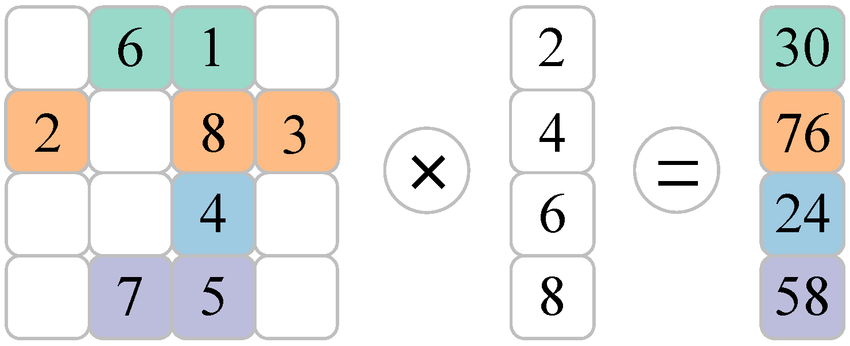
\includegraphics[width=0.28\textwidth]{spmv.png}
        \caption{SpMV multiplication}
        \label{fig:spmv}
    \end{wrapfigure}

    The product between a matrix $A$ of size $n \cdot m$ and a vector $x$
    (which \textbf{must be} of size $m$) gives as a result a vector $y$ of size
    $n$ as shown in figure \ref{fig:spmv}.

    The $i$-th element of the resulting vector can be calculated given the
    following formula:
    $$
    y_i = \sum\limits_{j = 0}^{m} A_{ij} x_j
    $$
    Where $y_i$ is the $i$-th element of the resulting vector.

    \section{Storage format}

    Storing a large sparse matrix as a dense one is not memory efficient at all
    since most of the values are zeros and therefore do not contribute to the
    final result.

    To store sparse matrices efficiently many storage formats were, and still
    are, being developed such as the \textbf{Compressed Sparse Row} matrix
    format, CSR in short.

    \begin{wrapfigure}{r}{0.3\textwidth}
        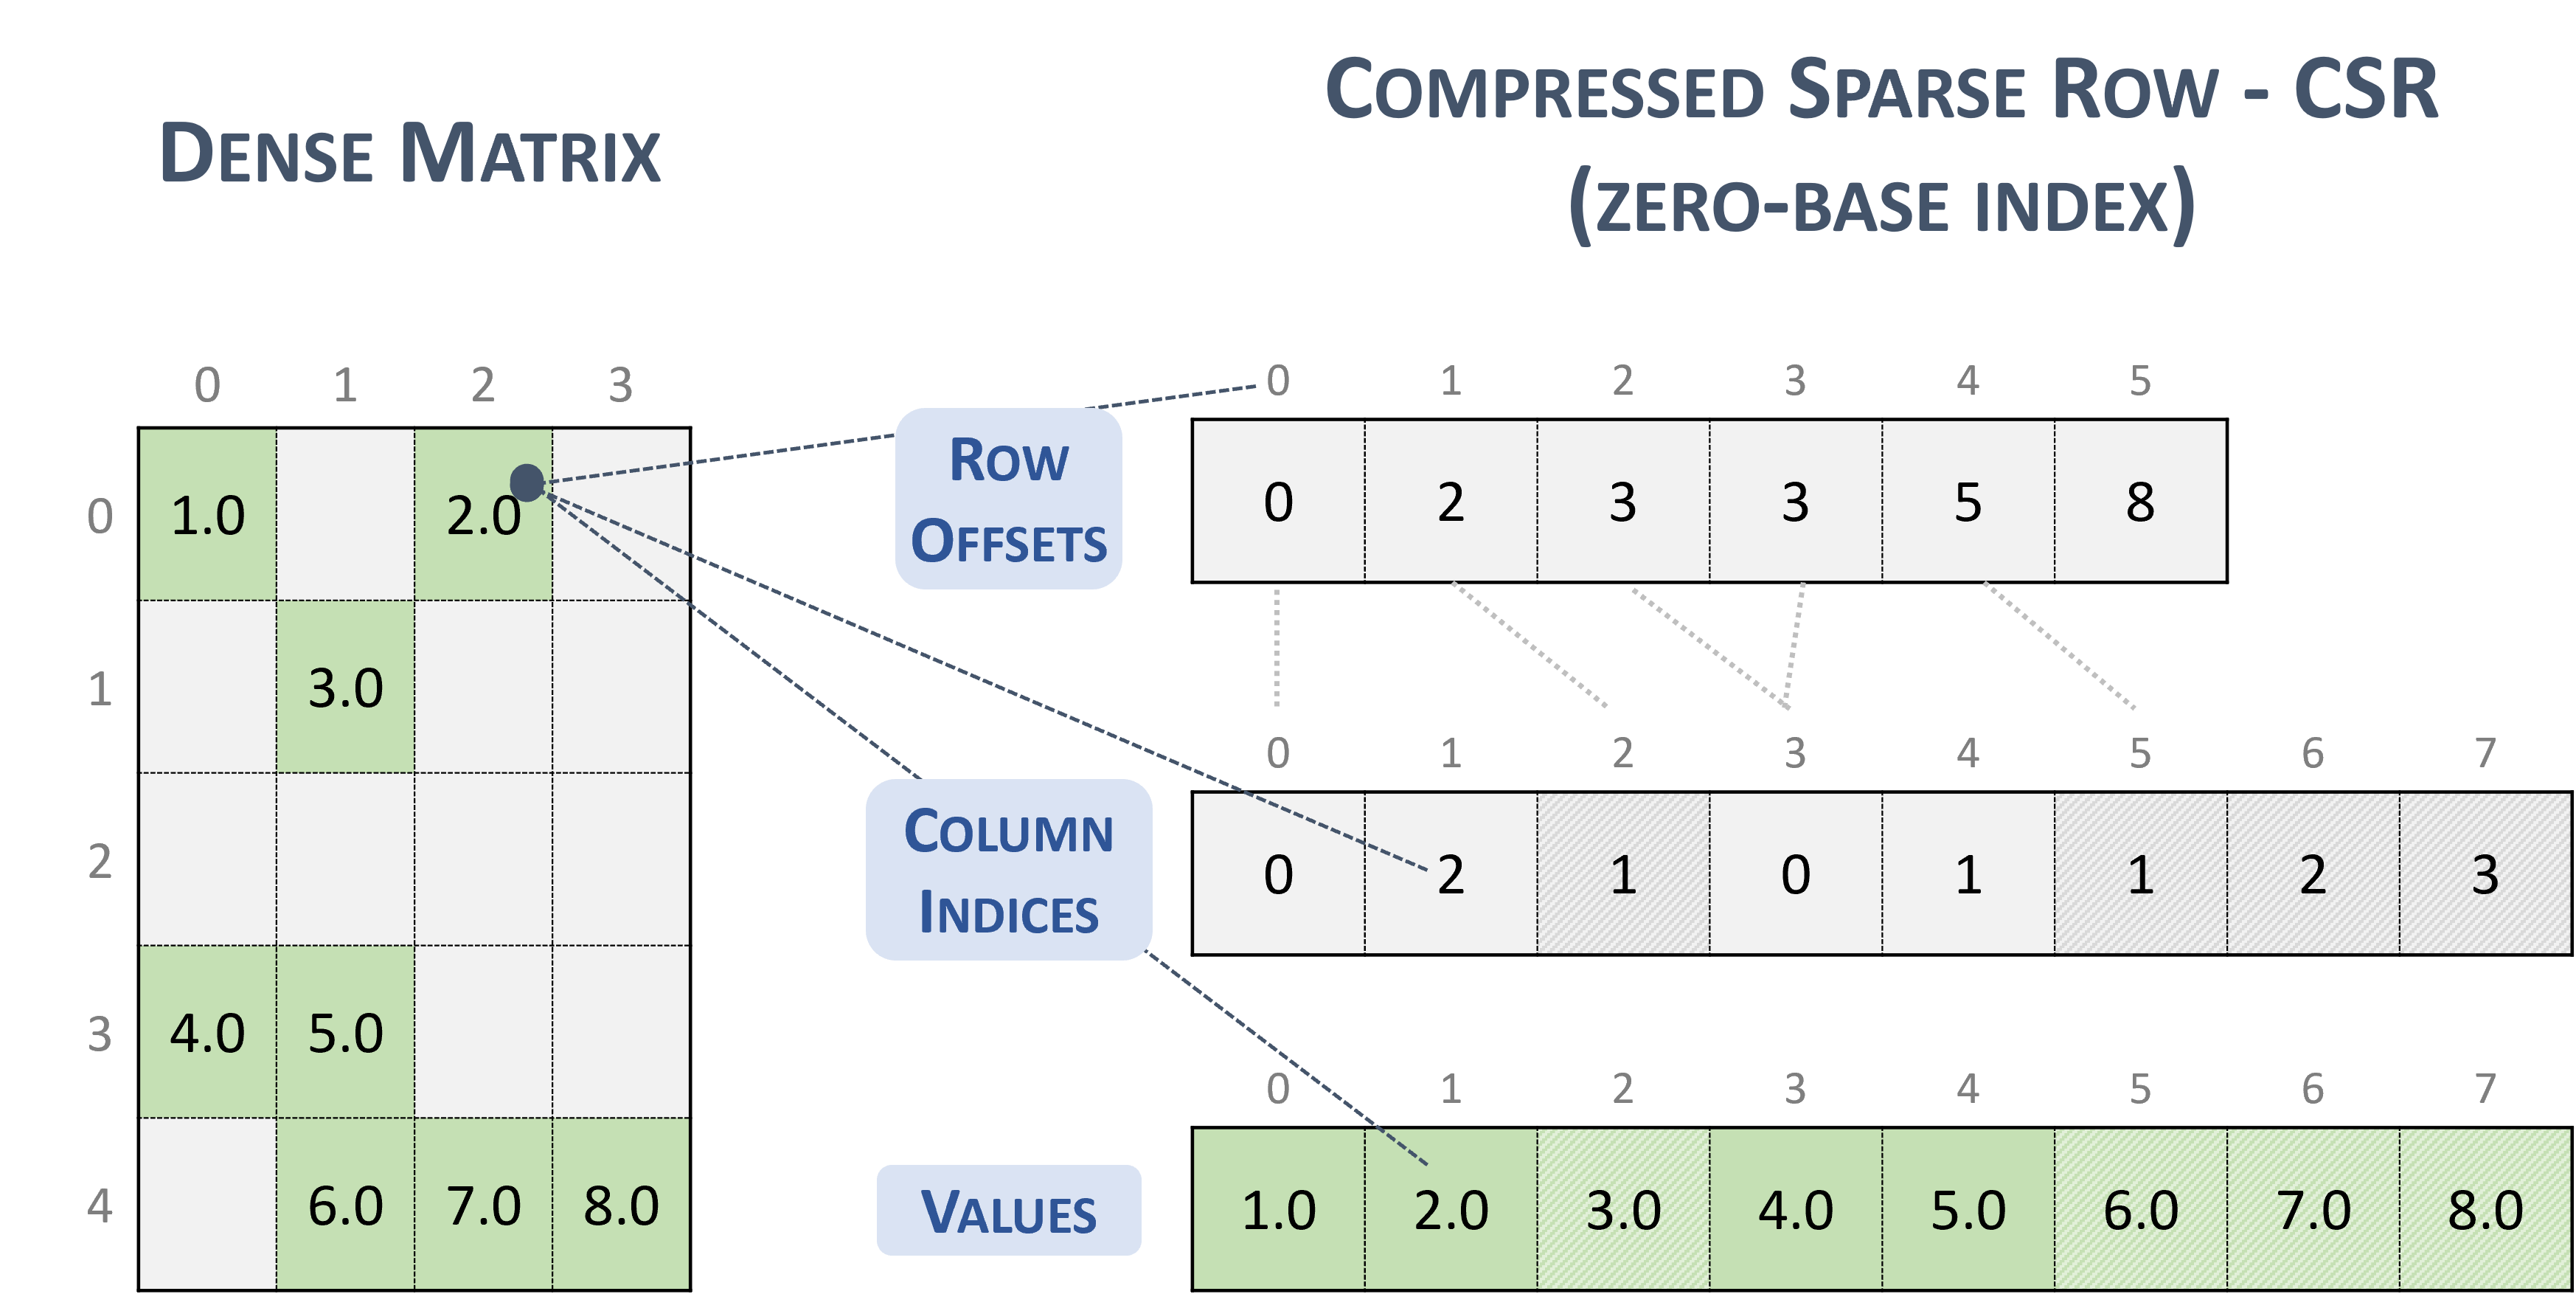
\includegraphics[width=0.3\textwidth]{csr-format.png}
        \caption{CSR matrix format}
        \label{fig:csr-format}
    \end{wrapfigure}

    This format consists of three arrays used to store the rows, columns and
    non-zero values of the matrix, the main advantage is that the array
    containing the row indices is constructed by sorting and creating a prefix
    sum of the original row indices reducing the length of the row array from
    the number of non-zero to the number of rows plus one.

    Using the CSR format, access to the $i$-th row can be obtained just by
    taking the $i$-th value of the row array as shown in figure
    \ref{fig:csr-format}.

    \section{State of the Art \& Related Work}

    As a starting point, the \textbf{Compressed Sparse Row} (CSR) format
    \cite{eisenstat1977csr} introduced in 1977 is used to store sparse matrices
    efficiently in memory.

    In the previous deliverable, we observed that simple implementations like
    \textbf{CSR-scalar}, which assigns one thread per row
    \cite{isupov2021spmvhp}, can exhibit highly variable performance depending
    on the input matrix's structure.
    In contrast, the baseline used for this work is the \textbf{Balanced CSR
    SpMV} approach \cite{flegar2017balancedcsr}, which offers improved
    robustness by being largely insensitive to the matrix's \textit{non-zero-
    per-row} distribution.
    This makes it more suitable for applying further optimizations.

    One of the two new implementations builds upon this balanced strategy by
    \textbf{adaptively} selecting among three different methods: CSR-stream,
    CSR-vector and CSR-vectorL, based on the non-zero density of each row
    \cite{daga2015adaptivesparse}, aiming to maximize performance under varying
    sparsity patterns.

    The second implementation is inspired by the CSR5 format \cite{liu2015csr5},
    which enhances parallelism by reorganizing the CSR data layout and
    leveraging \textbf{partial prefix sums}.
    In this approach, the matrix-vector product is divided into \textbf{fixed-size}
    blocks, within which partial prefix sums are computed.
    These are then efficiently reduced into final row-wise results using
    \textbf{shared memory}.
    This strategy minimizes redundant computations and significantly improves
    parallel efficiency, especially for matrices with irregular sparsity
    patterns.

    \section{Methodology and Implementation Strategy}\label{sec:methodology}

    For the \textbf{shared memory} optimized implementation, two separate CUDA
    kernels are used: one kernel performs \textbf{partial prefix sums} using
    shared memory, the second computes the final sum for each row, storing the
    result in the output vector.

    \begin{figure}[ht]
        \centering
        \begin{subfigure}{0.24\textwidth}
            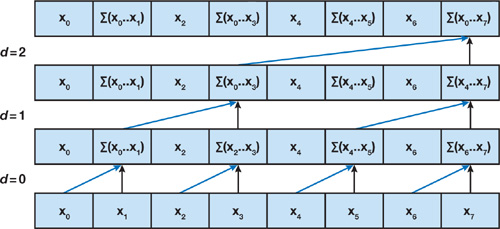
\includegraphics[width=\linewidth]{prefix-sum-up-sweep.jpg}
            \caption{Up-Sweep Phase (Reduce)}
            \label{fig:up-sweep}
        \end{subfigure}
        \hfill
        \begin{subfigure}{0.24\textwidth}
            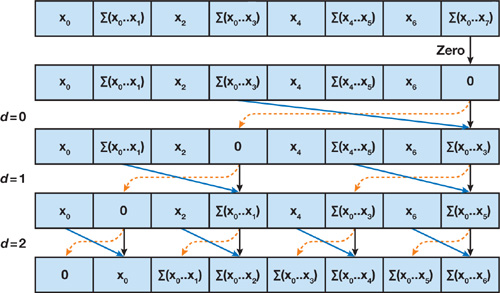
\includegraphics[width=\linewidth]{prefix-sum-down-sweep.jpg}
            \caption{Down-Sweep Phase}
            \label{fig:down-sweep}
        \end{subfigure}
        \caption{Parallel Prefix Sum}
        \label{fig:prefix-sum}
    \end{figure}

    The first kernel is launched with fixed-size blocks of 32 threads.
    Each thread computes the product between elements of the matrix and the
    input vector, storing the intermediate results in shared memory.

    As illustrated in Figure \ref{fig:prefix-sum}, a \textbf{parallel prefix
    sum} (scan) is performed using the technique described in \textit{GPU Gems
    3} \cite{harris2007prefixsum}.
    This method consists of two main stages: Up-Sweep (Reduction) and
    Down-Sweep, achieving faster prefix sum calculation.

    Once the prefix sum is computed for each block, the second kernel is used
    to calculate the final row sums.

    \begin{algorithm}[h!]
        \caption{Total sum}
        \algorithmicrequire~The input matrix $A$ and the output vector $y$.
        \begin{algorithmic}[1]
            \Procedure{SumAndStore}{$A$, $y$, $n$, $m$}
                \State $y \gets \emptyset$
                \State $sum \gets 0$

                \State \% Sum all the blocks values of the current row
                \For {$i \in row\_blocks$}
                    \State $sum = sum + A[i + block\_size - 1]$
                \EndFor

                \State \% Add missing values of the current row
                \If {$rows[tid + 1] \mod block\_size < block\_size$}
                    \State $sum = sum + A[rows[tid + 1] - 1]$
                \EndIf

                \State \% Subtract values of the previous row
                \If {$rows[tid] \mod block\_size > 0$}
                    \State $sum = sum - A[rows[tid] - 1]$
                \EndIf
                
                $y[tid] = sum$
                \State \textbf{return} $y$\Comment{the result vector}
            \EndProcedure
        \end{algorithmic}
        \label{alg:sum-and-store}
    \end{algorithm}

    To get the final result, \textbf{only the last element} of each row and of
    each block's prefix sum is copied back to global memory.
    This is sufficient, since prefix sums require only the values at the end of
    the current and previous range.
    Because each block computes its prefix sum independently, the last value in
    the block is \textbf{critical} for correctness.
    
    The second kernel is launched with one thread per row, which combines the
    prefix sum results to produce the final output vector.

    For the adaptive approach, \textbf{two auxiliary arrays} are generated to
    dynamically partition the matrix rows into processing groups.
    This partitioning is based on the number of non-zero (\textit{nnz})
    elements per row, aiming to \textbf{balance} the workload and improve
    efficiency.

    \begin{algorithm}[h!]
        \caption{Adaptive SpMV}
        \algorithmicrequire~Input matrix $A$, input vector $x$ and the auxiliary arrays $blocks$ and $meta$.
        \begin{algorithmic}[2]
            \Procedure{SpMV}{$A$, $x$, $y$, $n$, $m$, $blocks$, $meta$}
                \State $y \gets \emptyset$
                \State $rows \gets blocks[bid + 1] - blocks[bid]$\Comment{$bid$ is the block index}

                \If{$rows \ge NUM\_ROWS\_STREAM$}
                    \State{Execute CSR-Stream.}
                \ElsIf{$rows = 1$}
                    \State $start \gets blocks[bid]$
                    \State $nnz \gets rows[start + 1] - rows[start]$\Comment{$rows$ contains the matrix row indices}

                    \If{$nnz > NNZ\_PER\_WG$}
                        \State{Execute CSR-VectorL.}
                    \Else
                        \State{Execute CSR-Vector.}
                    \EndIf
                \EndIf

                \State \textbf{return} $y$\Comment{the result vector}
            \EndProcedure
        \end{algorithmic}
        \label{alg:SpMVrow}
    \end{algorithm}
 
    The number of processing groups (or GPU blocks) is determined during this
    preprocessing step.
    Each block uses a fixed number of threads to process its assigned range.

    Based on the size and density of each group, a different strategy is applied:
    \begin{itemize}
        \item \textbf{CSR-Stream}: Used for batches of multiple rows.
            It uses \textbf{scalar or logarithmic reduction} to process rows
            efficiently within a warp.
        \item \textbf{CSR-VectorL}: Used for single dense rows, utilizing
            multiple warps and atomic accumulation operations.
        \item \textbf{CSR-Vector}: Applied to single rows that are not dense
            enough to justify warp-level parallelism.
    \end{itemize}

    This adaptive strategy ensures \textbf{high performance} across matrices
    with varying row densities by applying the most suitable execution model
    per group. 

    \section{Experimental Setup \& Performance Analysis}
        \subsection{System Description}

        For the development of the project the following requirements were used
        inside the university cluster:
        \begin{itemize}
            \item SLURM 32.11.3
            \item CUDA 12.1
            \item GCC 12.3.0
            \item GNU Make 4.3
            \item OpenMP 17.0.6
            \item Eigen 12.3.0 (for the utilities)
            \item Python 3.9.18 (for the utilities) 
        \end{itemize}

        The project can be compiled using the provided Makefiles with GCC and
        CUDA compilers and can be run into the cluster via the SLURM workload
        manager utilities.

        \begin{table}[ht]
            \caption{System details}
            \label{tab:system_description}
            \centering
            \begin{adjustbox}{width=\columnwidth}
            \begin{tabular}{lllrl}
            \toprule
            \textbf{System} &  \textbf{Processor} & \textbf{Cores per Socket} & \textbf{RAM} & \textbf{Accelerator} \\
            \midrule
                laptop & Intel(R) Core(TM) i5-1035G1 CPU & 4 at 3.6 GHz & 8 GB & Intel Iris Plus Graphics G1 (Ice Lake) \\
                baldo & Intel(R) Xeon(R) Silver 4214 CPU & 12 at 2.2 GHz & 405 GB & \\
                edu-short & AMD EPYC 9334 32-Core Processor & 32 at 3.9 GHz & 810 GB & NVIDIA L40S \\
            \bottomrule
            \end{tabular}
            \end{adjustbox}
        \end{table}

        \subsection{Dataset description}
        
        \textbf{Eight} different matrices were selected as dataset, each with
        specific characteristics of size and sparsity to evaluate the
        performance of the various implementations in different scenarios.

        \begin{table}[ht]
            \caption{Matrix Details}
            \label{tab:matrix_details}
            \centering
            \begin{adjustbox}{width=\columnwidth}
            \begin{tabular}{lrrr|rr}
            \toprule
                \textbf{Name} & \textbf{Rows} & \textbf{Columns} & \textbf{Non-Zeros} & \textbf{Sparsity} & \textbf{Symmetric} \\
            \midrule
                \textbf{1138\_bus} & 1,138 & 1,138 & 4,054 & 99.69\% & Yes \\
                \textbf{bcsstk15} & 3,948 & 3,948 & 117,816 & 99.24\% & Yes \\
                \textbf{bcsstk31} & 35,588 & 35,588 & 1,181,416 & 99.91\% & Yes \\
                \textbf{pwtk} & 217,918 & 217,918 & 11,524,431 & 99.98\% & Yes \\
                \textbf{cage15} & 5,154,859 & 5,154,859 & 99,199,551 & 99.99\% & No \\
                \textbf{heart1} & 3,557 & 3,557 & 1,385,317 & 89.05\% & No \\
                \textbf{relat8} & 345,688 & 12,347 & 1,334,038 & 99.97\% & No \\
                \textbf{connectus} & 512 & 394,792 & 1,127,525 & 99.44\% & No \\
            \bottomrule
            \end{tabular}
            \end{adjustbox}
        \end{table}

        \subsection{Experimental Set-up}

    \section{Experimental Results}

    \section{Conclusion}

    \bibliographystyle{IEEEtran}
    \bibliography{references}

\end{document}
